\chapter{Derivation of nonlinear antenna stand model}\label{appendix:nonlinearAntennaStandModel}
The nonlinear model is based on the differential equations, as given in Equations \ref{eq:DCMotorFullMechanical} and \ref{eq:DCMotorLaplaceElectrical}. Equations \ref{eq:appendix:nonlinearDC-motorElecDone} and \ref{eq:appendix:nonlinearDC-motorMechDone} are given by doing the inverse laplace transform, since $\frac{d\Phi}{dt} = \omega_s(t)$.
\begin{subequations}
	\begin{align}
	v_{s}(t) = R_{a}\cdot i_a(t) + \frac{d i_a(t)}{d t}\cdot L_a + K_{e}\cdot\omega_{s}(t)\cdot N \addunit{\volt} \label{eq:appendix:nonlinearDC-motorElecDone}\\ 
\left( J_m\cdot N^2 + J_s\right)\cdot \frac{d \omega_s(t)}{d t} = K_t\cdot i_a(t)\cdot N -\left( B_m\cdot N^2 +B_s \right)\cdot \omega_s(t) \addunit{\newton\meter} \label{eq:appendix:nonlinearDC-motorMechDone}
	\end{align}
\end{subequations}

To simplify the model, a collective friction is defined $B = \left( B_m\cdot N^2 +B_s \right)$.

To derive a nonlinear model of the antenna stand, the friction coefficient $B$ must be modelled. By taking the data from \autoref{appendix:TJStandConstants}, a relationship between the current and angular velocity is given as in \autoref{appendix:tab:deriveNonlinearModelData}
\begin{table}[!h]
	\centering
	\caption{Some of the data from \autoref{appendix:TJStandConstants}. The angular frequencies are calculated values.}\label{appendix:tab:deriveNonlinearModelData}
	\begin{tabularx}{\textwidth}{XX}
	Current, $i_a(t)$ [\si{\milli\ampere}]	& Angular Frequency, $\omega_s(t)$ [\si{\radian\per\second}]						\\ \toprule \rowcolor{lightGrey}
		 30,7 & 1,05	\\
		 32,4 & 1,36 \\ \rowcolor{lightGrey}
		 35,8 & 2,09 \\
		 37,2 & 2,62 \\ \rowcolor{lightGrey}
		 40,8 & 3,04 \\
		 43,6 & 3,77\\ 
	\end{tabularx}
\end{table}

As the measurements were done in steady-state $\left[ \left( J_m\cdot N^2 + J_s\right)\cdot \frac{d \omega_s(t)}{d t} = 0 \right]$, the friction can be calculated by \autoref{eq:appendix:nonlinearFriction}, derived from \autoref{eq:appendix:nonlinearDC-motorMechDone}.
\begin{equation}
B =\frac{K_t\cdot i_a(t)\cdot N}{\omega_s (t)} \addunit{\newton\meter\second\per\radian}\label{eq:appendix:nonlinearFriction}
\end{equation}

By running the numbers in \autoref{appendix:tab:deriveNonlinearModelData}, a set of friction coefficients, dependent on the angular velocity $\omega_s(t)$ is acquired. The correlation between the friction coefficient and the angular velocity can be described as a decreasing power function as given in \autoref{eq:appendix:nonlinearFrictionModel}.
\begin{equation}
B(\omega_s(t))=\frac{0.05956}{\omega_s(t)^{0.73165}} \addunit{\newton\meter\second\per\radian} \label{eq:appendix:nonlinearFrictionModel}
\end{equation}
\startexplain
\explain{$B$ is the collective friction coefficient of the motor and stand}{\si{\newton\meter\second\per\radian}}
\stopexplain

From the \autoref{eq:appendix:nonlinearFrictionModel} it is seen that the friction coefficient increases exponentially as $\omega_s(t)$ goes towards zero. This would cause the simulation to accelerate a lot slower than the actual physical stand, and the friction coefficient is therefore approximated as \autoref{eq:appendix:nonlinearFrictionModelApproximated}.
\begin{align} \label{eq:appendix:nonlinearFrictionModelApproximated}
 B(\omega_s(t)) &=
  \begin{cases}
	\SI{0.1}{\newton\meter\radian\per\second}   															& \text{for} \left|\omega_s(t)\right| < 0.5 \\
	\frac{0.05956}{\omega_s(t)^{0.73165}} \si{\newton\meter\radian\per\second}		& \text{for} \left|\omega_s(t)\right| \geq 0.5
  \end{cases}
\end{align}

From \autoref{appendix:TJStandConstants} it is noted that the stand does not move before voltages above $V_{start} = \SI{1.76}{\volt}$ is applied to the motor. This behaviour is modelled by applying a dead-zone to the velocity, and zeroing all resultant torques below a specific threshold, equivalent to the torque needed to start rotation, if the stand is not rotating. The torque is modelled first, then the velocity dead-zone is calculated.

Assuming steady-state and $\omega_s(t) = 0$, the torque required to start rotation can be calculated by combining Equations \ref{eq:appendix:nonlinearDC-motorElecDone} and \ref{eq:appendix:nonlinearDC-motorMechDone}, and is given by \autoref{eq:appendix:nonlinearNeededTorque}. The values of $K_t$, $N$ and $R_a$ is taken from \autoref{tab:TechAnalDCMotorConstants}.
\begin{equation} \label{eq:appendix:nonlinearNeededTorque}
\tau_{start} = \frac{V_{start} \cdot K_t \cdot N}{R_a} = \SI{0.10489}{\newton\meter}
\end{equation}
\startexplain
\explain{$\tau_{start}$ is torque needed to start rotation}{\si{\newton\meter}}
\explain{$V_{start}$ is the voltage needed to start rotation}{\si{\volt}}
\stopexplain

The resultant torque is therefore modelled as \autoref{eq:appendix:nonlinearTorqueApproximation}.
\begin{align} \label{eq:appendix:nonlinearTorqueApproximation}
\tau_{res} &=
  \begin{cases}
	0   		& \text{if } \omega_s(t) = 0 \text{ and } \tau < \SI{0.10489}{\newton\meter} \\
	\tau		& \text{if } \omega_s(t) \neq 0 \text{ or } \tau \geq \SI{0.10489}{\newton\meter}
  \end{cases}
\end{align}
\startexplain
\explain{$\tau$ is the torque applied in the linear model}{\si{\newton\meter}}
\explain{$\tau_{res}$ is the resultant torque in the nonlinear model}{\si{\newton\meter}}
\stopexplain

To calculate the span of the velocity dead-zone, it is assumed that the applied torque is linear, and the torque $\tau_{start} = \SI{0.10489}{\newton\meter}$ is applied to the antenna stand. If the friction coefficient still follows \autoref{eq:appendix:nonlinearFrictionModelApproximated}, the resultant velocity can be calculated by combining Equations \ref{eq:appendix:nonlinearDC-motorElecDone} and \ref{eq:appendix:nonlinearDC-motorMechDone}, and assuming steady-state. The span of the dead-zone is therefore given by \autoref{eq:appendix:nonlinearVelocityDeadzone}.
\begin{equation} \label{eq:appendix:nonlinearVelocityDeadzone}
\omega_{dz} = \frac{V_{start}\cdot K_t \cdot N}{K_e\cdot K_t\cdot N^2+ B(\omega_{dz})\cdot R_a} = \SI{0.40266}{\radian\per\second}
\end{equation}

The resultant angular velocity of the stand is therefore modelled as specified in \autoref{eq:appendix:nonlinearResultantVelocity}
\begin{align} \label{eq:appendix:nonlinearResultantVelocity}
\omega_{sres}(t) &=
  \begin{cases}
	0   		& \text{if } \left| \omega_s(t) \right | < \omega_{dz} \\
	\omega_s(t) - \text{sign}[\omega_s(t)] \cdot \omega_{dz}		& \text{if } \left| \omega_s(t) \right | \geq \omega_{dz}
  \end{cases}
\end{align}
\startexplain
\explain{$\omega_s(t)$ is the torque applied in the linear model}{\si{\newton\meter}}
\explain{$\omega_{sres}(t)$ is the resultant torque in the non linear model}{\si{\newton\meter}}
\stopexplain

Using the models of the friction coefficient $B(\omega_{res}(t))$, resultant torque $\tau_{res}$, and resultant velocity $\omega_{res}(t)$, a model for the full feedback control system, as illustrated on \autoref{design:fig:controlSystemAzimuth} in \autoref{sec:introToDesign} can be assembled in MATLAB Simulink, as illustrated on \autoref{fig:appendix:antennaStandSimulink}.

\begin{figure}[p]
	\centering
	%The figure is slightly wider than the textheight, because it looks better
	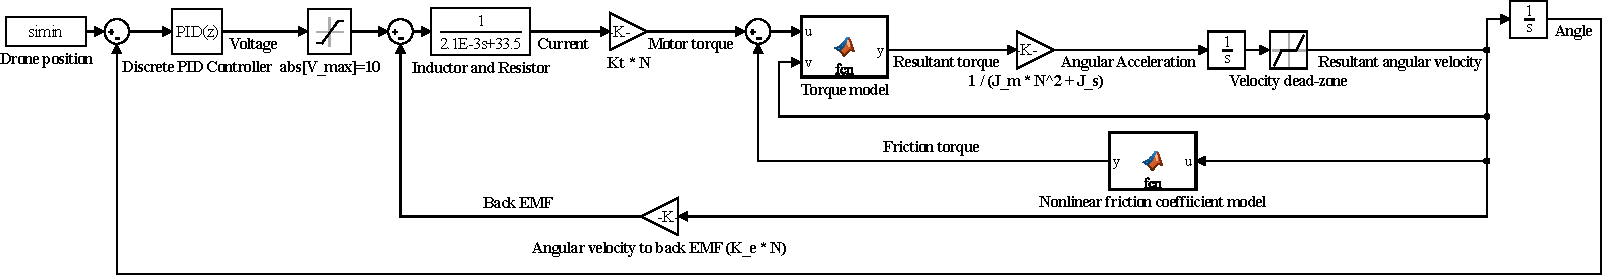
\includegraphics[width=\textheight+100pt, angle=90]{figures/appendix/nonlinearStandModel/antennaStandSimulink}
	\caption{Model of the antenna stand, for azimuth rotation, made in MATLAB Simulink.}
	\label{fig:appendix:antennaStandSimulink}
\end{figure}
